%-----------------------------------------------------------------------------
% DOCUMENT CLASS
%-----------------------------------------------------------------------------
%\documentclass[12pt,a4paper,twoside,pdftex]{book}

% Put a comment on next line to output single-sided version
\def\twopage{1}

\ifx\twopage\undefined
  % Single-sided document
  \documentclass[12pt,a4paper,oneside,pdftex]{book}
\else
  % Double-sided document
 \documentclass[12pt,a4paper,twoside,pdftex]{book}
\fi

\pdfcompresslevel=9
%-----------------------------------------------------------------------------
% PACKAGES
%-----------------------------------------------------------------------------

\usepackage[italian, english]{babel}    % Last language is default one
\usepackage{graphicx} 
\usepackage[utf8]{inputenc}

\usepackage{url} 
\usepackage{amssymb} 
\usepackage{eurosym} 
\usepackage{subfig}
\usepackage{enumerate}
\usepackage{xtab}
\usepackage{fancyvrb}
\usepackage{sverb}
\usepackage{comment}
\usepackage{booktabs}
\usepackage{amsmath}
\usepackage{graphicx}
\usepackage{multirow}
\usepackage{longtable}
\usepackage{color}
\usepackage{microtype}
\usepackage{algorithm}
\usepackage[noend]{algpseudocode}
\usepackage[square, numbers, comma, sort&compress]{natbib} % Use the natbib reference package - read up on this to edit the reference style; if you want text (e.g. Smith et al., 2012) for the in-text references (instead of numbers), remove 'numbers' 
\usepackage{hyperref}
\hypersetup{
    colorlinks,
    citecolor=black,
    filecolor=black,
    linkcolor=black,
    urlcolor=black
}

% Enhance verbatim style
\RecustomVerbatimEnvironment
  {verbatim} {Verbatim}
  {gobble=2, frame=lines}
\CustomVerbatimEnvironment
  {verbatim2} {Verbatim}
  {gobble=2}


%-----------------------------------------------------------------------------
% HEADERS AND FOOTERS
%-----------------------------------------------------------------------------


\usepackage{fancyhdr}
\pagestyle{fancy}

\renewcommand{\chaptermark}[1]{\markboth{#1}{}}
\renewcommand{\sectionmark}[1]{\markright{\thesection\ #1}}
% Remove footer text
\fancyhf{}

% Setup header and footer
\ifx\twopage\undefined
  % Single-sided document
  \fancyhead[R]{\bfseries\thepage}
  \fancyhead[L]{\bfseries\leftmark}
\else
  % Double-sided document
  \fancyhead[LE,RO]{\bfseries\thepage}
  \fancyhead[RE]{\bfseries\leftmark}
  \fancyhead[LO]{\bfseries\rightmark}
\fi

% Setup header and footer rules
\renewcommand{\headrulewidth}{0.5pt}
\renewcommand{\footrulewidth}{0pt}
\addtolength{\headheight}{0.5pt}
\fancypagestyle{plain}{
  \fancyhead{}
  \renewcommand{\headrulewidth}{0pt}
}
\setlength{\headheight}{14.5pt}


%-----------------------------------------------------------------------------
% PAGE MARGINS
%-----------------------------------------------------------------------------

\ifx\twopage\undefined
  % Single-sided document
  \addtolength{\oddsidemargin}{0cm} 
  \addtolength{\textwidth}{1.5cm}
  \addtolength{\headwidth}{1.5cm}
  \addtolength{\textheight}{1cm}
\else
  % Double-sided document
  \addtolength{\evensidemargin}{-2.0cm}
  \addtolength{\oddsidemargin}{.5cm}
  \addtolength{\textwidth}{1.5cm}
  \addtolength{\headwidth}{1.5cm}
  \addtolength{\textheight}{1cm}
\fi


%-----------------------------------------------------------------------------
% LEADING
%-----------------------------------------------------------------------------

\usepackage{setspace}
\onehalfspacing

%-----------------------------------------------------------------------------
% EQUATIONS
%-----------------------------------------------------------------------------



%-----------------------------------------------------------------------------
% DOCUMENT
%-----------------------------------------------------------------------------

\begin{document}
\newcommand{\rood}[1]{\textcolor{red}{[#1]}} 
\newcommand{\pending}[1]{\textcolor{cyan}{[#1]}}
%\newcommand{\ok}[1]{\textcolor{green}{[#1]}} 

% Choose Phys. Rev. style for bibliography
\bibliographystyle{unsrt}
% \nocite{*}   % to show non cited biblio

%------------------------------------------------ Cover page
\frontmatter
\thispagestyle{empty}

\begin{center}

	\textsc{Politecnico di Milano}\\
 	Scuola di Ingegneria dell'Informazione\\  

 	\par\vskip 0.2cm

 	
\includegraphics[width=7cm]{figures/polimi_logo.png}\\
  
 	\par\vskip 0.2cm  
  
  	\textsc{Polo territoriale di Como}\\
  	Master of Science in Computer Engineering\\  


  	\par\vskip 2cm
  	
\LARGE{ \bf	ECG-ira: An efficient mobile app for ECG analysis}


		
\end{center}

\par\vskip 1.5cm

\begin{flushleft}
  	\textbf{Supervisor}: Prof. Giuseppe Pozzi\\
  	\textbf{Co-Supervisors}: Ulisse Pizzagalli, Dr. Rodolfo Pizzuto \\
    \textbf{Assistant Supervisor}: 	\dots\dots\dots\dots\dots\dots \\
\end{flushleft}

\par\vskip 1cm

\begin{flushleft}
  	\textbf{Master Graduation Thesis by}: \\
  	Antonello Fodde - 817371 \\ 
  	Chai Botta - 817333 \\  
\end{flushleft}

\par\vskip 1cm

\begin{center}
 	Academic Year 2015-2016
\end{center}






% For double-sided document, leave a blank page
\ifx\twopage\undefined
\else
  \newpage \thispagestyle{empty} \null \newpage
\fi

%------------------------------------------------ Inscription

% Page without header
%\thispagestyle{empty} \null
%\vspace{4cm}
%\begin{flushright}
%\emph{Essentially, \\ all models are wrong, \\but some are useful.\\}
%\emph{\textit{\\(George E. P. Box)}}
%\end{flushright}

%------------------------------------------------ Abstract

% Page without header
\newpage \thispagestyle{empty} \newpage 
\chapter{Abstract}

Lorem ipsum dolor sit amet, consectetur adipiscing elit. Curabitur malesuada suscipit nisl, vitae gravida odio imperdiet a. Etiam sed auctor tellus. Donec sed mauris eget nibh luctus accumsan. Sed imperdiet purus in elit iaculis, non commodo nisl varius. Integer sit amet diam laoreet, viverra lacus id, placerat nisl. Aenean ultricies sollicitudin elit in sodales. Vivamus euismod eleifend justo, ac pellentesque risus. Donec eleifend, justo a pharetra laoreet, est dolor condimentum nulla, nec auctor ligula justo eget diam. Mauris augue eros, elementum quis vulputate eget, ullamcorper eget mauris.
Maecenas quis hendrerit velit. Donec vehicula dictum tellus, et aliquam sem viverra maximus. Maecenas gravida purus quis dui vulputate ornare. Morbi ac orci ut nunc tristique ultricies nec mattis massa. In imperdiet nisl ut risus faucibus, ut semper libero egestas. Nam imperdiet ullamcorper nunc, eu dictum felis dapibus a. Aliquam nec ante posuere, tristique dui semper, hendrerit erat. Nunc purus massa, lobortis a laoreet vel, posuere sit amet nisl. Duis ut viverra nisl. Pellentesque habitant morbi tristique senectus et netus et malesuada fames ac turpis egestas.

Nulla elit risus, efficitur condimentum erat id, laoreet ullamcorper tellus. Nam non rutrum massa. Suspendisse vitae mauris vitae arcu elementum molestie et at diam. Proin efficitur vehicula ligula, id rhoncus dui pulvinar et. Nunc nec ultrices nunc, ut cursus libero. Donec mattis vehicula ex eget efficitur. Ut tellus arcu, vehicula nec ullamcorper ut, vulputate eu arcu. In cursus ut justo non sodales. Sed massa urna, eleifend eu nisi eget, tincidunt efficitur nibh. Donec at molestie arcu. Duis elementum lectus at tristique scelerisque. Donec sodales purus viverra urna interdum, sit amet convallis velit lacinia. Aliquam mollis tempus rhoncus. Quisque ultricies nisi quis metus rhoncus mattis.
In fermentum facilisis tristique. Fusce ultricies quam id suscipit venenatis. Vestibulum hendrerit nibh eget ligula tristique, a tincidunt metus viverra. Aliquam finibus dui velit, a accumsan lacus tempus sit amet. Fusce in justo lorem. Mauris a porttitor justo, eget tincidunt erat. Ut quis semper risus. Aliquam eu malesuada metus. Aliquam erat volutpat. Sed ac diam finibus, pellentesque enim ut, commodo mi. Nam ligula odio, semper eget diam id, tempus cursus risus. Donec viverra, elit quis molestie ultrices, odio risus ornare orci, at eleifend nisl risus elementum tellus. Cum sociis natoque penatibus et magnis dis parturient montes, nascetur ridiculus mus. Suspendisse eu aliquet est, scelerisque vulputate justo.

Suspendisse egestas posuere lacinia. Integer non mi maximus, rhoncus massa eu, aliquam risus. Nam nisl nisi, semper nec efficitur eu, tincidunt vel justo. Sed vestibulum tristique consequat. Phasellus sodales nunc quis pharetra mattis. Pellentesque eu fermentum sem, vel efficitur odio. Suspendisse consectetur turpis et nisi viverra commodo. Quisque ornare porta nisi, eget aliquam nisl interdum sed. Nulla elementum quam sit amet enim mollis, in rhoncus felis lacinia. Nam vel justo purus. Nulla pellentesque ex in eros rutrum tincidunt. Morbi consequat felis a libero dictum, vel malesuada est dignissim. Maecenas diam lacus, laoreet ut quam vel, pharetra aliquet nisi. Suspendisse auctor aliquam odio eu tincidunt. Aenean lacinia semper diam. Suspendisse potenti.

\chapter{Sommario}
Negli ultimi anni il mercato della healthcare ha mantenuto una forte tendenza di interesse e subito un rapido sviluppo. Questo sviluppo ha sfruttato tutte le potenzialità rese disponibili dalle ultime tecnologie mobile: sono numerose le aziende che si sono specializzate nella creazione di dispositivi proprietari che svolgessero una determinata funzione: si va da quelli che fornissero supporti per il mondo del fitness, come l’analisi della massa corporea o del battito cardiaco, a quelli focalizzati nel campo medicale, come i sensori di pressione sanguigna o di livello di glucosio. Molti di questi hanno come potenzialità l’alta caratteristica di interfacciamento con l’utente, attraverso l’uso di mobile app che si sincronizzino con questi dispositivi e che analizzino i dati al fine di presentarli all’utente nel modo più accessibile possibile.\\
Il nostro lavoro vuole inserirsi in questo ambito, più specificatamente in quello medicale. Il nostro progetto nasce dal lavoro di alcuni studenti che ci hanno preceduto, e si presenta come una sua evoluzione in chiave moderna. Questo ci ha permesso di avere, come punto di partenza, un dispositivo e un software PC (precedentemente sviluppati) con cui interfacciarci. In particolare, il primo è un dispositivo di acquisizione di segnale ECG (elettrocardiogramma), chiamato ZEcg. La sua particolarità è rappresentata dalle ridotte dimensioni e dal suo interfacciamento di connessione, che sfrutta la tecnologia bluetooth, e quindi senza fili. Il software invece, nasce precedentemente, alle origini come software PC di visualizzazione ed analisi di aritmie di tracciati ECG. Successivamente è stato riadattato, al fine di aggiungere come funzionalità l’acquisizione in tempo reale dal dispositivo ZEcg di tracciati ECG.\\
Sfruttando il dispositivo ZEcg e gli algoritmi di analisi del precedente software, il progetto ha come fine la creazione di una mobile app per smartphone e tablet, che diventi un vero e proprio supporto per un medico specializzato, e che quindi fornisca tutte le funzionalità necessarie per acquisire, visualizzare ed analizzare un tracciato ECG. Inoltre l’app dovrà essere progettata per una massima estensibilità e compatibilità con più dispositivi mobile. Le caratteristiche di adattamento e rapidità che l’applicazione dovrà avere come primi obbiettivi, ci hanno portato al nome “ECG-ira”, che sta per “ECG-instantaneous responsive analyzer”. \\
Nel corso dei capitoli si analizzeranno i problemi riscontrati e le scelte implementative che hanno portato alla realizzazione del prodotto finale.




%\newpage \thispagestyle{empty} \newpage 
%\chapter{Abstract}

Lorem ipsum dolor sit amet, consectetur adipiscing elit. Curabitur malesuada suscipit nisl, vitae gravida odio imperdiet a. Etiam sed auctor tellus. Donec sed mauris eget nibh luctus accumsan. Sed imperdiet purus in elit iaculis, non commodo nisl varius. Integer sit amet diam laoreet, viverra lacus id, placerat nisl. Aenean ultricies sollicitudin elit in sodales. Vivamus euismod eleifend justo, ac pellentesque risus. Donec eleifend, justo a pharetra laoreet, est dolor condimentum nulla, nec auctor ligula justo eget diam. Mauris augue eros, elementum quis vulputate eget, ullamcorper eget mauris.
Maecenas quis hendrerit velit. Donec vehicula dictum tellus, et aliquam sem viverra maximus. Maecenas gravida purus quis dui vulputate ornare. Morbi ac orci ut nunc tristique ultricies nec mattis massa. In imperdiet nisl ut risus faucibus, ut semper libero egestas. Nam imperdiet ullamcorper nunc, eu dictum felis dapibus a. Aliquam nec ante posuere, tristique dui semper, hendrerit erat. Nunc purus massa, lobortis a laoreet vel, posuere sit amet nisl. Duis ut viverra nisl. Pellentesque habitant morbi tristique senectus et netus et malesuada fames ac turpis egestas.

Nulla elit risus, efficitur condimentum erat id, laoreet ullamcorper tellus. Nam non rutrum massa. Suspendisse vitae mauris vitae arcu elementum molestie et at diam. Proin efficitur vehicula ligula, id rhoncus dui pulvinar et. Nunc nec ultrices nunc, ut cursus libero. Donec mattis vehicula ex eget efficitur. Ut tellus arcu, vehicula nec ullamcorper ut, vulputate eu arcu. In cursus ut justo non sodales. Sed massa urna, eleifend eu nisi eget, tincidunt efficitur nibh. Donec at molestie arcu. Duis elementum lectus at tristique scelerisque. Donec sodales purus viverra urna interdum, sit amet convallis velit lacinia. Aliquam mollis tempus rhoncus. Quisque ultricies nisi quis metus rhoncus mattis.
In fermentum facilisis tristique. Fusce ultricies quam id suscipit venenatis. Vestibulum hendrerit nibh eget ligula tristique, a tincidunt metus viverra. Aliquam finibus dui velit, a accumsan lacus tempus sit amet. Fusce in justo lorem. Mauris a porttitor justo, eget tincidunt erat. Ut quis semper risus. Aliquam eu malesuada metus. Aliquam erat volutpat. Sed ac diam finibus, pellentesque enim ut, commodo mi. Nam ligula odio, semper eget diam id, tempus cursus risus. Donec viverra, elit quis molestie ultrices, odio risus ornare orci, at eleifend nisl risus elementum tellus. Cum sociis natoque penatibus et magnis dis parturient montes, nascetur ridiculus mus. Suspendisse eu aliquet est, scelerisque vulputate justo.

Suspendisse egestas posuere lacinia. Integer non mi maximus, rhoncus massa eu, aliquam risus. Nam nisl nisi, semper nec efficitur eu, tincidunt vel justo. Sed vestibulum tristique consequat. Phasellus sodales nunc quis pharetra mattis. Pellentesque eu fermentum sem, vel efficitur odio. Suspendisse consectetur turpis et nisi viverra commodo. Quisque ornare porta nisi, eget aliquam nisl interdum sed. Nulla elementum quam sit amet enim mollis, in rhoncus felis lacinia. Nam vel justo purus. Nulla pellentesque ex in eros rutrum tincidunt. Morbi consequat felis a libero dictum, vel malesuada est dignissim. Maecenas diam lacus, laoreet ut quam vel, pharetra aliquet nisi. Suspendisse auctor aliquam odio eu tincidunt. Aenean lacinia semper diam. Suspendisse potenti.


%------------------------------------------------ Lists

% Pages without header
\newpage \thispagestyle{empty} \newpage 
\tableofcontents

\newpage \thispagestyle{empty} \newpage 
\listoffigures

%\newpage \thispagestyle{empty} \newpage 
%\listofalgorithms
%\listofmyequations

%\newpage \thispagestyle{empty} \newpage 
%\listoftables
\newpage \thispagestyle{empty} \newpage 

%------------------------------------------------ Main matters

\mainmatter

% Chapter 1

\chapter{Introduction}
\label{Chapter1} 

ECG-ira stands for ECG (electrocardiogram) instant rapid analyzer and it is an android application developed for the acquisition, visualization and analysis of the electrocardiogram signals. The application acquires and stores  the record from the zecg acquisition device  (using the zecg device format) property of the Politecnico of Milan but it can also open and visualize other ecg format from other  devices. Ecg-ira is part of a greater and long term project (zecg itself was part of a first step). ECG-ira aims to exploit the reliability and performance of a complex software for electrocardiogram signal acquisition,  visualization  and processing within a smartphone device through a mobile application. Apart of the analysis algorithm already implemented during a past thesis (by Diego Ulisse Pizzagalli), the application was designed and implemented from scratch. During the process we dealt with the devices limitation in term of performance power and limited memory. We overcome many issues, related also to small and different screen size and density of pixel, due to the great number of different devices currently on the market. We had to exploit the multithreading and efficient memory usage strategies in order to achieve responsiveness and fulfill the medical requirement for an ECG compliant application. The result is an application which is easy to use because it follows all the best design principles according to the official Google guidelines for responsive UI and UX. By taking advantage of the multithreading capabilities and the usage of all the available cores into a device, we achieved an application which performs fast and well.\\
This thesis is structured as follows: 
\begin{itemize}
	\item After this introduction we give a brief but detailed overview about the heart, its functionalities and how an electrocardiogram is related to it by explaining starting from what it is an ecg to how heart electrical signals are detected and read.
	\item In the State of Art chapter we show the panorama of the actual devices for an ecg acquisition and some available applications on the market which allow to open and read an ecg record.
	\item Then it follows the Objective chapter in which we describe and explain the goal of this thesis work.
	\item The Requirements chapter is where we list functional and nonfunctional sets of features which came up during the planning phase. The final result should be compliant with all of them.
	\item The Problem chapter deals with all the issues related to the project development. Here we discussed about the problem of choosing a development platform with respect to another, the hardware limitation on a smartphone device and the problems strictly related to the ecg signals.
	\item The Solution choices chapter is where we explain and provide our reasonings to the implementation choices, from the platform choice to the programming language choice to why we decided to avoid using drawings libraries preferring a custom and proprietary implementation.
	\item In the System architecture chapter we provide a general overview of the project structure for both the acquisition device implementation and architecture both the mobile application structure and main functionalities.
	\item In the Implementation details chapter we described all the main components and Java classes. Here we provide also hints for future implementations and adaptations.
	\item In the Final result chapter we propose some screenshots, with descriptive captions and descriptions of the main screens of the application; then we go through a performance analysis of application by observing how it affects the memory, the cpu and the response time of some portion of the code. The tests were conducted on many different devices but only data from the older devices (2011) and the newest (November 2015) are compared.
	\item In the Conclusion chapter we sum up the overall results giving an overview of what has been done and providing some post considerations about the work done.
	\item In the Future works chapter we provide hints for further implementations in order to make ECG-ira really an all in one solution as an ECG mobile application. We also put our consideration on the future of the mobile software with respect to the desktop one, according to the new trends and the fact that the mobile environments is penetrating even more in our daily lives and can really positively change the way patients are connected with the health care providers.
\end{itemize}
% Chapter 2

\chapter{Electrocardiography overview}
\label{Chapter2} 

This chapter will introduce some basic but fundamental concepts about electrocardiography starting from the heart to the ECG and all issues related to the topic. We will start introducing the heart, its functionality and the entire circulatory system.\\
After that we will describe in details the electrical activity inside the heart and how heart beats are generated. Following there will be a description of the electrocardiogram and the ECG signals. In the last section of this chapter we will discuss about all the noises and interference related to the ECG signal during its acquisition. 

\section{The heart}
This chapter’s focus is to describe in details the human heart. We will start from the structure to end up describing the heart functionality.

\subsection{Human heart structure}
The human heart is an organ that pumps blood throughout the body via the circulatory system, supplying oxygen and nutrients to the tissues and removing carbon dioxide and other wastes.\\
This fundamental organ has four chambers: two upper chambers(the atrial) and two lower ones(the ventricles). The right atrium and the right ventricle together make up the “right heart”, and the left atrium and left ventricle make up the”left heart”. The two sides of the heart are separated by a muscle called the septum. \\
A double-walled sac called the pericardium, encases the heart, which serves to protect the heart and anchors it inside the chest. Between the outer layer, the parietal pericardium, and the inner layer, the serous pericardium, runs pericardial fluid, which lubricates the heart during contractions and movements of the lungs and diaphragm.
The heart outer wall consists of three layers. The outermost wall layer, or epicardium, is the inner wall of the pericardium.  The middle layer, or myocardium, contains the muscle that contracts. The inner layer, or endocardium, is the lining that contacts the blood.\\
The tricuspid valve and the mitral valve make up the atrioventricular (AV) valves, which connect the atria and the ventricles. The pulmonary semilunar valve separates the right ventricle from the pulmonary artery, and the aortic valve separates the left ventricle from the aorta. The heartstrings, or chordae tendineae, anchor the valves to heart muscles.\\
The sinoatrial node produces the electrical pulses that drive heart contractions.\\
\begin{figure}[ht!]
\centering
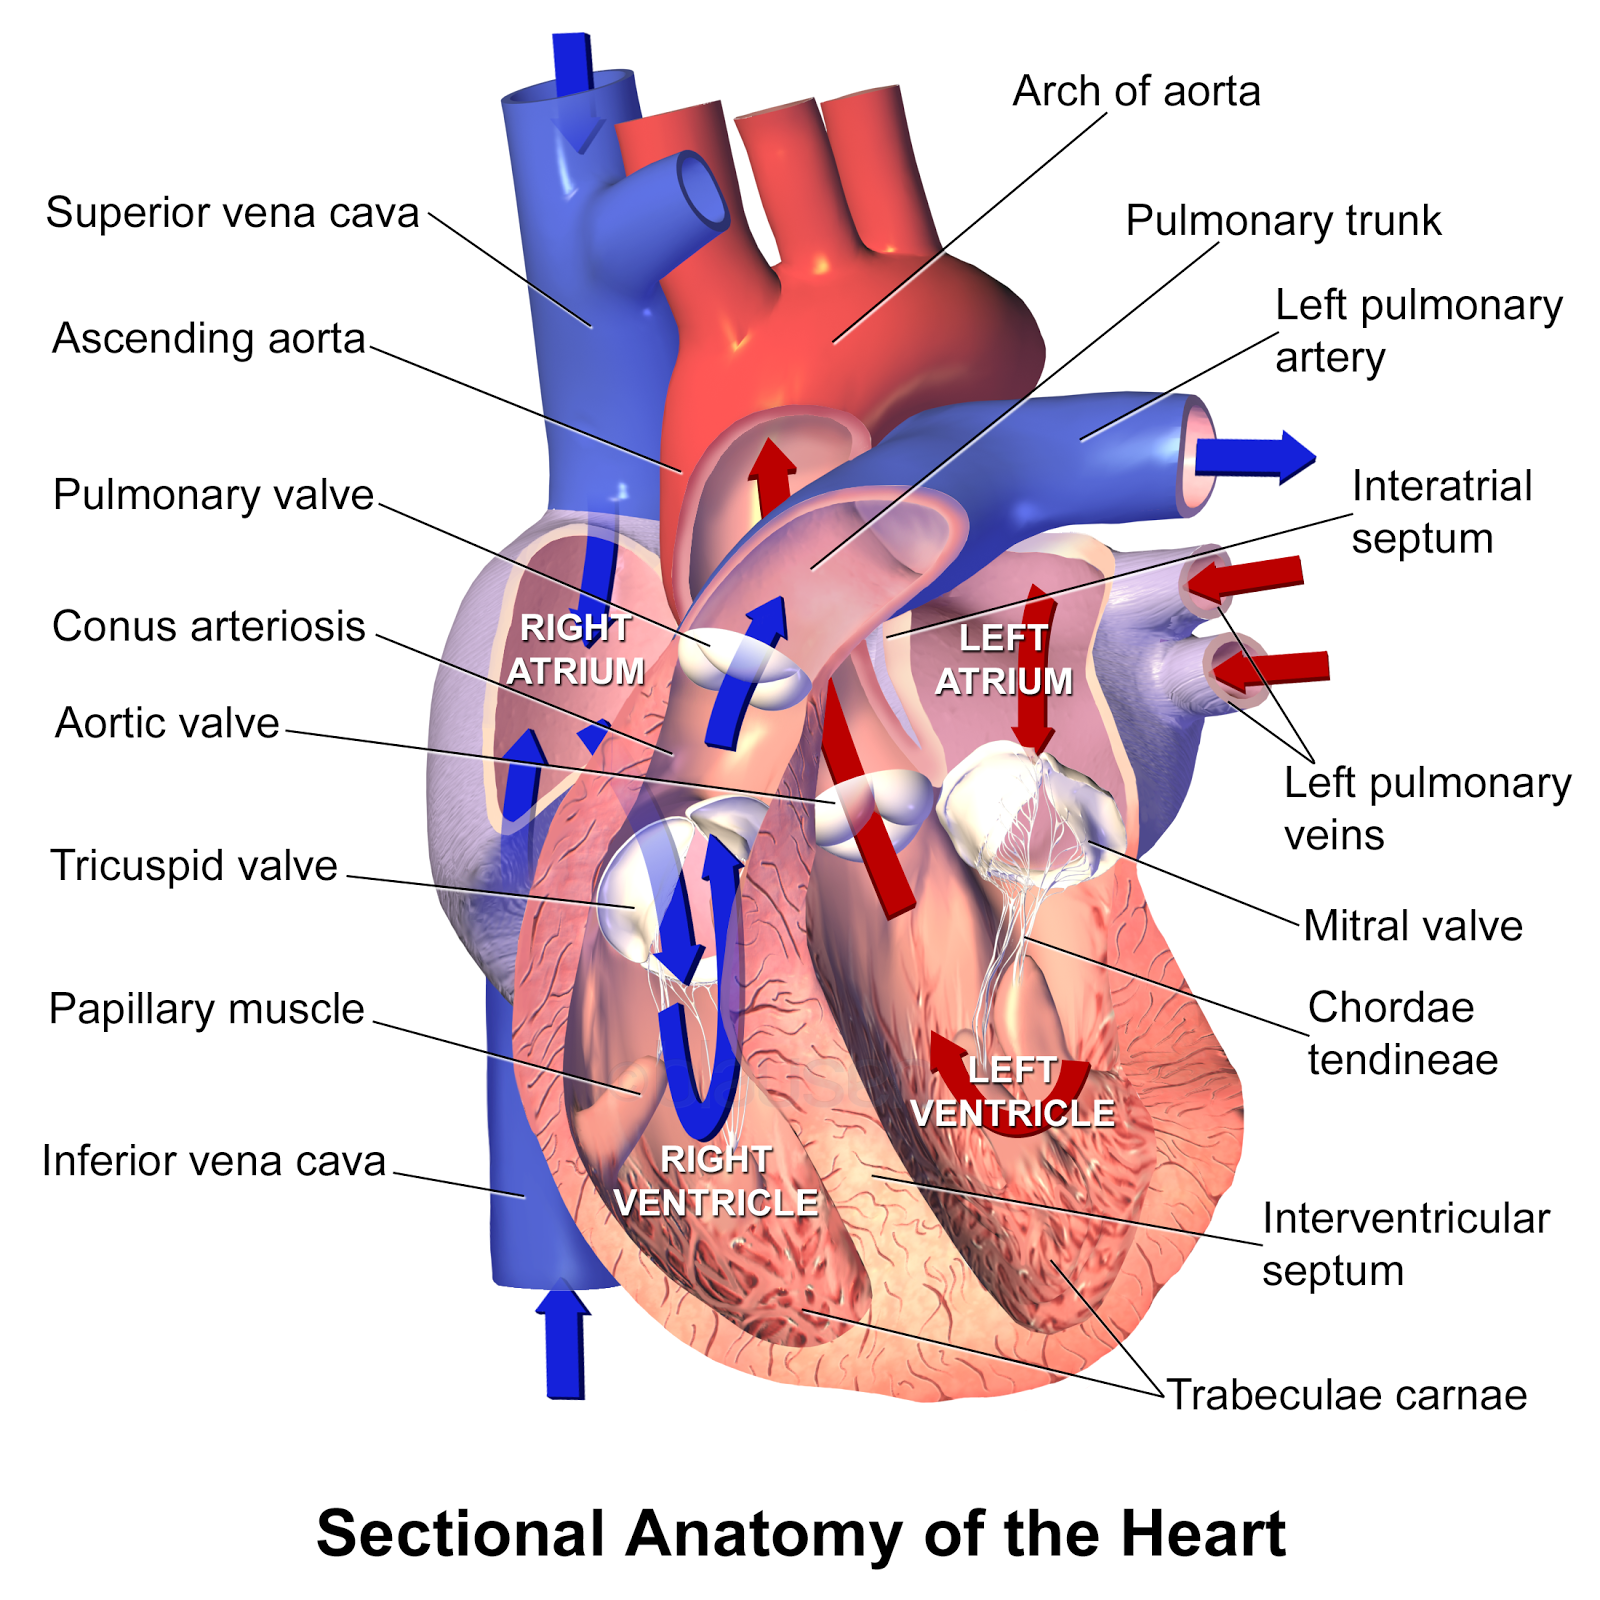
\includegraphics[width=100mm]{figures/ch2/1.png}
\caption{The human heart structure.\cite{ref1}}
\label{fig2.1}
\end{figure}

\subsection{Human heart function}
The heart circulates blood through two pathways: the pulmonary circuit and the systemic circuit.\\
In the pulmonary circuit, deoxygenated blood leaves the right ventricle of the heart via the pulmonary artery and travels to the lungs, then returns as oxygenated blood to the left atrium of the heart via the pulmonary vein.\\
In the systemic circuit, oxygenated blood leaves the body via the left ventricle to the aorta, and from there enters the arteries and capillaries where it supplies the body's tissues with oxygen. Deoxygenated blood returns via veins to the venae cavae, re-entering the heart's right atrium.\\
Of course, the heart is also a muscle, so it needs a fresh supply of oxygen and nutrients too. After the blood leaves the heart through the aortic valve, two sets of arteries bring oxygenated blood to feed the heart muscle. The left main coronary artery, on one side of the aorta, branches into the left anterior descending artery and the left circumflex artery. The right coronary artery branches out on the right side of the aorta.\\
Blockage of any of these arteries can cause a heart attack, or damage to the muscle of the heart. A heart attack is distinct from cardiac arrest, which is a sudden loss of heart function that usually occurs as a result of electrical disturbances of the heart rhythm. A heart attack can lead to cardiac arrest, but the latter can also be caused by other problems.\\
The heart contains electrical "pacemaker" cells, which cause it to contract — producing a heartbeat.\\
Each cell has the ability to be the 'band leader' and have everyone follow. In people with an irregular heartbeat, or atrial fibrillation, every cell tries to be the band leader, which causes them to beat out of sync with one another.\\
A healthy heart contraction happens in five stages:
\begin{enumerate}
	\item In the first stage (early diastole), the heart is relaxed.
	\item Then the atrium contracts (atrial systole) to push blood into the ventricle.
	\item Next, the ventricles start contracting without changing volume.
	\item Then the ventricles continue contracting while empty.
	\item Finally, the ventricles stop contracting and relax.
\end{enumerate}
Then the cycle repeats.\\
Valves prevent backflow, keeping the blood flowing in one direction through the heart.\\
\\
Some interesting data about the human heart are:
\begin{itemize}
	\item A human heart is roughly the size of a large fist.
	\item The heart weighs between about 280 to 340 grams in men and 230 to 280 grams in women.
	\item The heart beats about 100,000 times per day (about 3 billion beats in a lifetime).
	\item An adult heart beats about 60 to 80 times per minute.
	\item Newborns' hearts beat faster than adult hearts, about 70 to 190 beats per minute.
	\item The heart pumps about 6 quarts (5.7 liters) of blood throughout the body.
	\item The heart is located in the center of the chest, usually pointing slightly left
\end{itemize}
\begin{figure}[ht!]
	\centering
	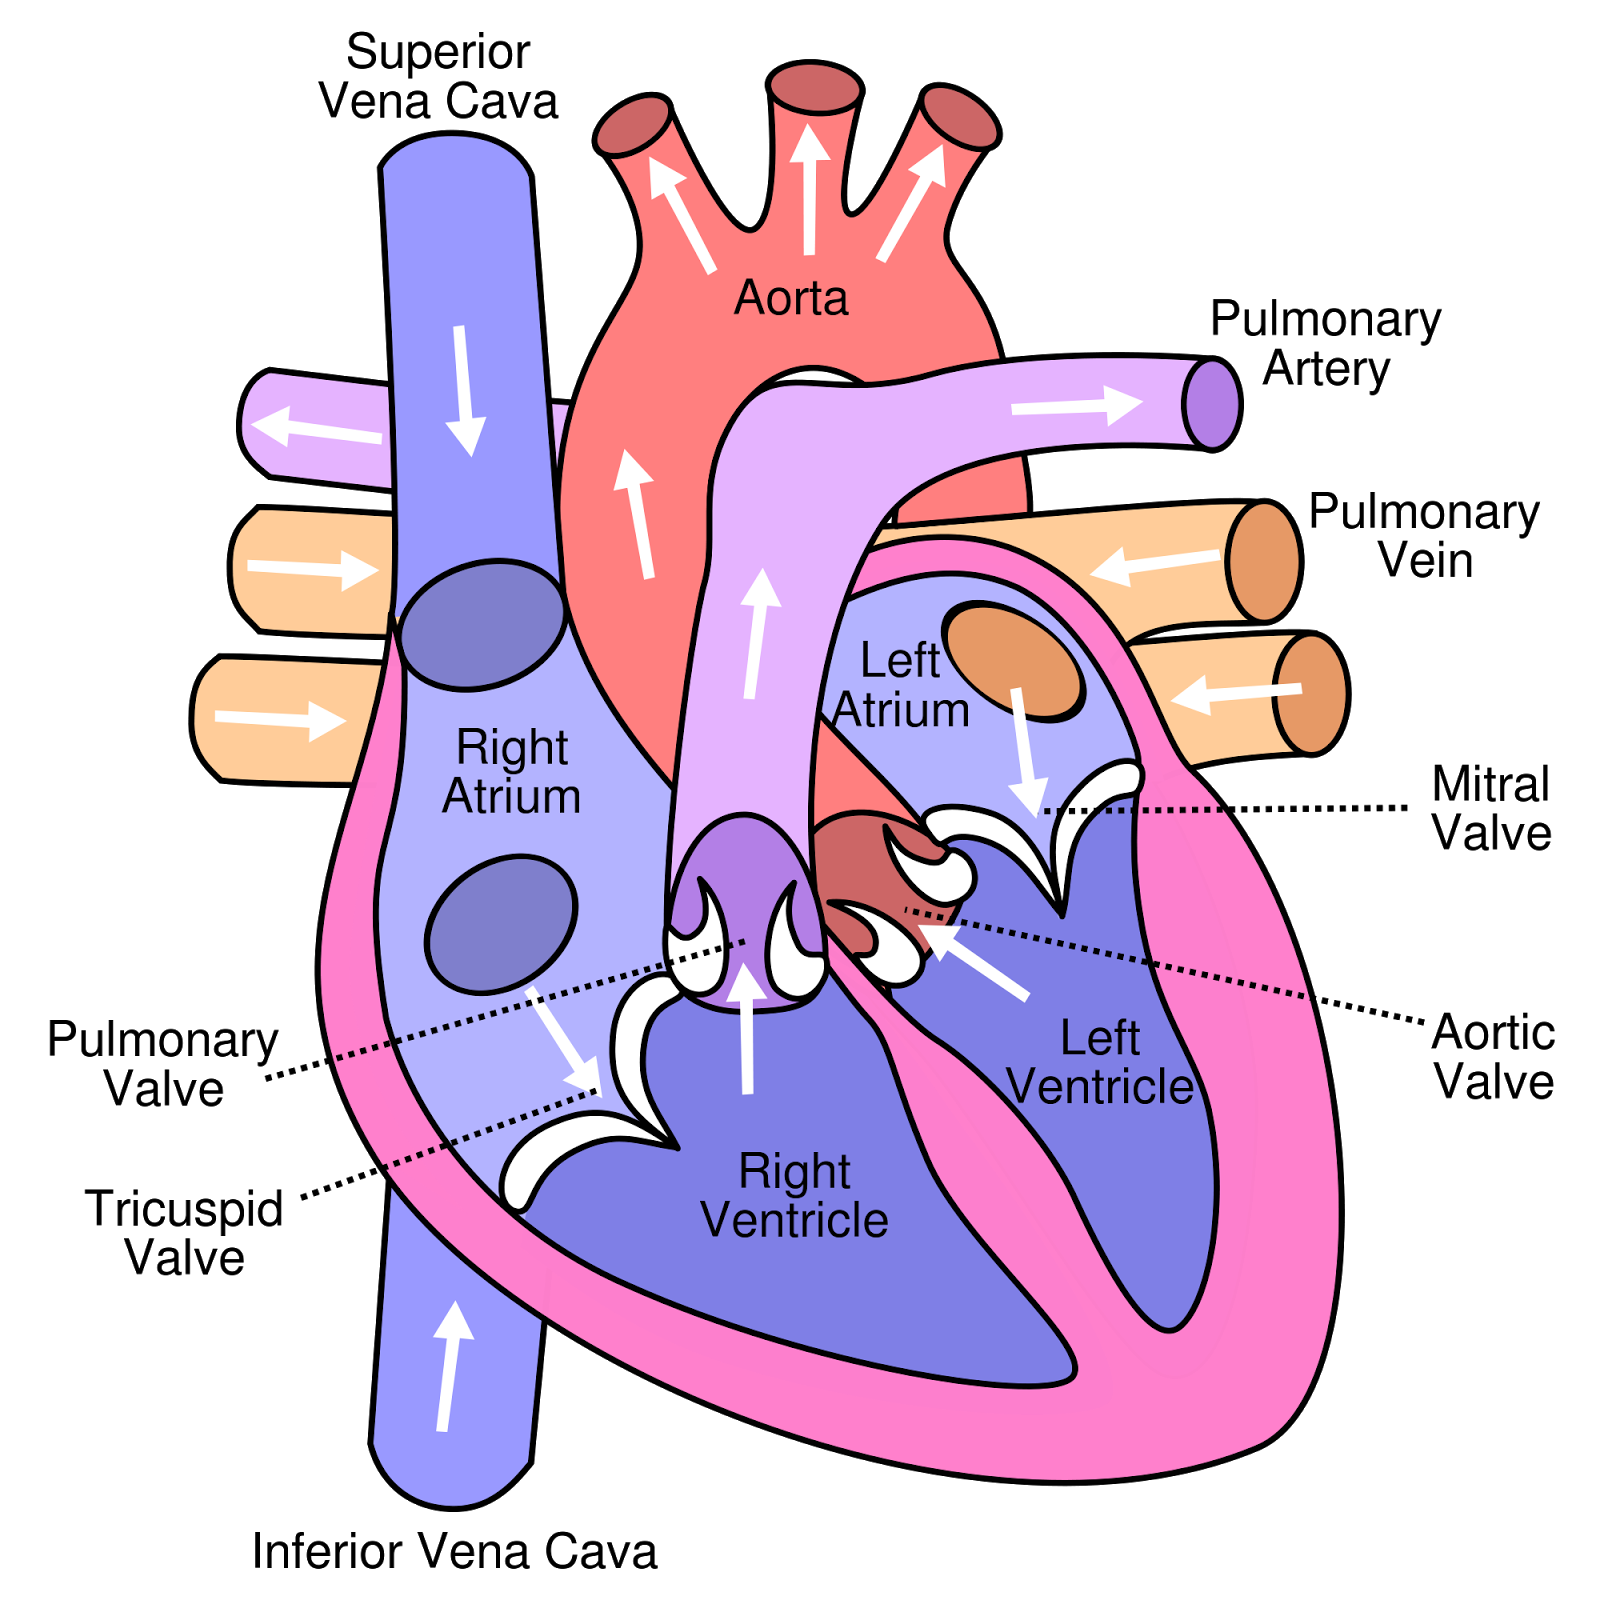
\includegraphics[width=90mm]{figures/ch2/2.png}
	\caption{The circulatory system with blood flow.}
	\label{fig2.2}
\end{figure}

\section{Heart electrical activity}
The heart has a natural pacemaker that regulates the pace or rate of the heart. It sits in the upper portion of the right atrium (RA) and is a collection of specializes electrical cells known as the SINUS or SINOATRIAL (SA) node.\\
Like the spark-plug of an automobile it generates a number of "sparks" per minute. Each "spark" travels across a specialized electrical pathway and stimulates the muscle wall of the four chambers of the heart to contract (and thus empty) in a certain sequence or pattern. The upper chambers or atria are first stimulated. This is followed by a slight delay to allow the two atria to empty. Finally, the two ventricles are electrically stimulated. In an car, the number of sparks per minute generated by a spark plug is increased when you press the gas pedal or accelerator. This revs up the motor. In case of the heart, adrenaline acts as a gas pedal and causes the sinus node to increase the number of sparks per minute, which in turn increases the heart rate. The release of adrenaline is controlled by the nervous system. The heart normally beats at around 72 times per minute and the sinus node speeds up during exertion, emotional stress, fever, etc., or whenever our body needs an extra boost of blood supply. In contrast, it slows down during rest or under the influence of certain medications. Well trained athletes also tend to have a slower heart beat.\\

\begin{figure}[ht!]
	\centering
	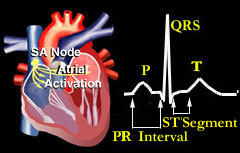
\includegraphics[width=60mm]{figures/ch2/3.png}
	\caption{The SA node fires and electrical impulses travels through the right and left atrium. \label{overflow}}
	\label{fig2.3}
\end{figure}
\begin{figure}[ht!]
	\centering
	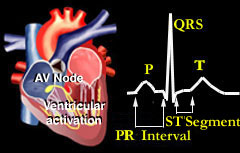
\includegraphics[width=60mm]{figures/ch2/4.png}
	\caption{The impulse then move to the ventricular area.}
	\label{fig2.4}
\end{figure}

The sequence of electrical activity within the heart is displayed in the diagrams above and occurs as follows:
\begin{enumerate}
	\item As the SA node fires, each electrical impulse travels through the right and left atrium. This electrical activity causes the two upper chambers of the heart to contract. This electrical activity and can be recorded from the surface of the body as a "P" wave" on the patient's EKG or ECG (electrocardiogram).
	\item The electrical impulse then moves to an area known as the AV (atrio-ventricular) node. This node sits just above the ventricles. Here, the electrical impulse is held up for a brief period. This delay allows the right and left atrium to continue emptying its blood contents into the two ventricles. This delay is recorded as a "PR interval." The AV node thus acts as a "relay station" delaying stimulation of the ventricles long enough to allow the two atria to finish emptying.
	\item Following the delay, the electrical impulse travels through both ventricles (via special electrical pathways known as the right and left bundle branches). The electrically stimulated ventricles contract and blood is pumped into the pulmonary artery and aorta. This electrical activity is recorded from the surface of the body as a "QRS complex". The ventricles then recover from this electrical stimulation and generates an "ST segment" and T wave on the ECG.
\end{enumerate}

\section{Electrocardiogram}
An electrocardiogram(abbreviated as ECG or EKG) is a test that measures the electrical activity of the heartbeat. With each beat, an electrical impulse (or wave) travels through the heart. This wave causes the muscle to squeeze and pump blood from the heart. A normal heartbeat on ECG will show the timing of the top and lower chambers.\\
The right and left atria or upper chambers make the first wave called a “P wave" following a flat line when the electrical impulse goes to the bottom chambers. The right and left bottom chambers or ventricles make the next wave called a “QRS complex." The final wave or “T wave” represents electrical recovery or return to a resting state for the ventricles.\\
\begin{figure}[ht!]
	\centering
	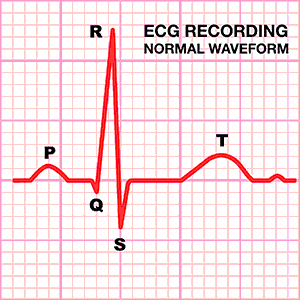
\includegraphics[width=60mm]{figures/ch2/5.png}
	\caption{An example of a normal ECG waveform. }
	\label{fig2.5}
\end{figure}
Each waves in the figure 2.5 is no other than the result of different views or perspectives of the waveforms generated from the current in the heart.\\
There are two type of ECGs recordings: the 12-lead ECG  and the rhythm strip. Both give valuable information about heart function.\\
We will focus our attention on the 12-lead ECG. It records information from 12 different views of the heart and provides a complete picture of electrical activity. The limb leads and the chest, or precordial, leads reflect information from the different planes of the heart. Different leads provide different information. The six limb leads I, II, III, augmented vector right (aVR), augmented vector left (aVL), and augmented vector foot (aVF) provide information about the heart’s frontal (vertical) plane. Leads I, II, and III require a negative and positive electrode for monitoring, which makes those leads bipolar. The augmented leads record information from one lead and are called unipolar.\\
The six precordials or V leads V1, V2, V3, V4, V5, and V6 provide information about the heart’s horizontal plane. Like the augmented leads, the precordial leads are also unipolar, requiring only a single electrode. The opposing pole of those leads is the center of the heart as calculated by the ECG.\\
The position of the leads are crucial for a right ECG recordings. It is common to use the so called Einthoven’s triangle, a set of positions to set up standard limb leads.
\begin{figure}[ht!]
	\centering
	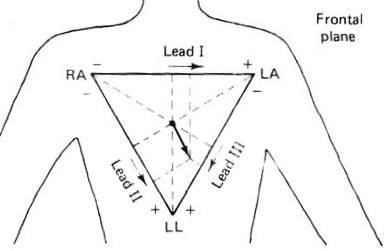
\includegraphics[width=80mm]{figures/ch2/6.png}
	\caption{The Einthoven’s triangle show the right position to place leads over the chest.}
	\label{fig2.6}
\end{figure}
The electrodes for leads I, II, III are about equidistant from the heart and form an equilateral triangle.

\subsection{Lead I}
It provides a view of the heart that shows current moving from right to left. Because the current flows from negative to positive, the positive electrode for this lead is placed on the left arm or on the left side of the chest; the negative electrode is placed on the right arm. Lead I produces a positive deflection on ECG tracings and is helpful in monitoring atrial and hemiblock.

\subsection{Lead II}
Lead II produces a positive deflection. Place the positive electrode on the patient’s left leg and the negative electrode on the right arm. For continuous monitoring, place the electrodes on the torso for convenience, with the positive electrode below the lowest palpable rib at the left midclavicular line and the negative electrode below the right clavicle. The current travels down and to the left in this lead. Lead II tends to produce a positive, high voltage deflection, resulting in tall P, R, and T waves. This lead is commonly used for routine monitoring and is useful for detecting sinus node and atrial arrhythmias.

\subsection{Lead III}
Lead III produces a positive deflection. The positive electrode is placed on the left leg; the negative electrode, on the left arm. Along with lead II, this lead is useful for detecting changes associated with an inferior wall myocardial infarction. The axes of the three bipolar limb leads I, II, and III form a triangle around the heart and provide a frontal plane view of the heart.

\subsection{Augmented leads}
Leads aVR, aVL, and aVF are called augmented leads. They measure electrical activity between one limb and a single electrode. Lead aVR provides no specific view of the heart. Lead aVL shows electrical activity coming from the heart’s lateral wall. Lead aVF shows electrical activity coming from the heart’s inferior wall.

\subsection{Precordials leads}
The six unipolar precordial leads (V1, V2, V3, V4, V5  and V6) are placed in sequence across the chest and provide a view of the heart’s horizontal plane.
\begin{itemize}
	\item Lead V1—The precordial lead V1 electrode is placed on the right side of the sternum at the fourth intercostal rib space. This lead corresponds to the modified chest lead MCL1 and shows the P wave, QRS complex, and ST segment particularly well. It helps to distinguish between right and left ventricular ectopic beats that result from myocardial irritation or other cardiac stimulation outside the normal conduction system. Lead V1 is also useful in monitoring ventricular arrhythmias, ST-segment changes, and bundle-branch blocks.
	\item Lead V2—Lead V2 is placed at the left of the sternum at the fourth intercostal rib space.
	\item  Lead V3—Lead V3 goes between V2 and V4. Leads V1, V2, and V3 are biphasic, with both positive and negative deflections. Leads V2 and V3 can be used to detect ST-segment elevation.
	\item Lead V4—Lead V4 is placed at the fifth intercostal space at the midclavicular line and produces a biphasic waveform.
	\item Lead V5—Lead V5 is placed at the fifth intercostal space at the anterior axillary line. It produces a positive deflection on the ECG and, along with V4, can show changes in the ST segment or T wave.
	\item Lead V6—Lead V6, the last of the precordial leads, is placed level with V4 at the midaxillary line. This lead produces a positive deflection on the ECG.
\end{itemize}
\begin{figure}[ht!]
	\centering
	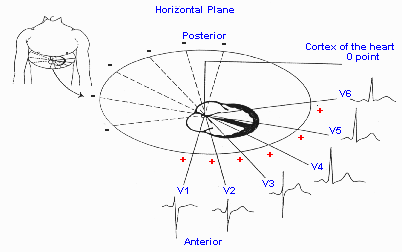
\includegraphics[width=90mm]{figures/ch2/7.png}
	\caption{Precordial leads and their position related to the heart and the chest horizontal plane.}
	\label{fig2.7}
\end{figure}

\subsection{How to read a ECG record}
Waveforms produced by the heart’s electrical current are recorded on graphed ECG paper by a stylus. An ECG paper consists of horizontal and vertical lines forming a grid. A piece of ECG paper is called an ECG strip or tracing.
\begin{figure}[ht!]
	\centering
	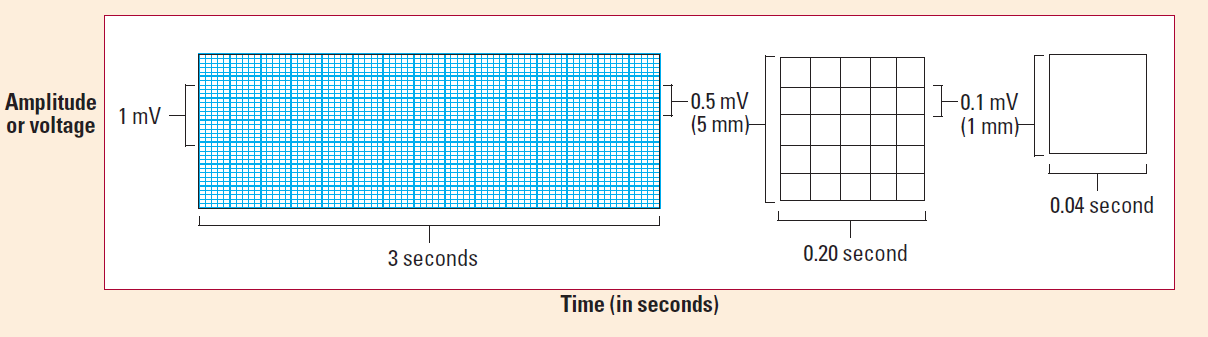
\includegraphics[width=130mm]{figures/ch2/8.png}
	\caption{A typical ECG paper.}
	\label{fig2.8}
\end{figure}
The horizontal axis of the ECG strip represents time. Each small block equals 0.04 second, and five small blocks form a large block, which equals 0.2 second. This time increment is determined by multiplying 0.04 second (for one small block) by 5, the number of small blocks that compose a large block. Five large blocks equal 1 second (5 x 0.2). When measuring or calculating a patient’s heart rate, a 6-second strip consisting of 30 large blocks is usually used. The ECG strip’s vertical axis measures amplitude in millimeters (mm) or electrical voltage in millivolts (mV). Each small block represents 1 mm or 0.1 mV; each large block, 5 mm or 0.5 mV. To determine the amplitude of a wave, segment, or interval, count the number of small blocks from the baseline to the highest or lowest point of the wave, segment, or interval.

\section{Noises and interferences}
Obtaining a reliable ECG recording is still an issue. In fact there may occur many problems interfering with the signals. Some of these problems include artifacts from patient movement and poorly placed or poorly functioning equipment.

\subsection{Artifact}
Artifact , also called waveform interference, may be seen with excessive movement (somatic tremor). The baseline of the ECG appears wavy, bumpy, or tremulous. Dry electrodes may also cause this problem to occur due to poor contact.
\begin{figure}[ht!]
	\centering
	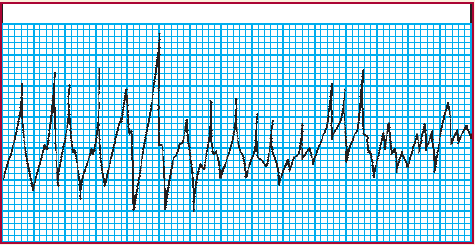
\includegraphics[width=90mm]{figures/ch2/9.png}
	\caption{ECG waveform interference due to artifact may cause monitoring to fail due to unreadable signals.}
	\label{fig2.9}
\end{figure}

\subsection{Interference}
Electrical interference, also called 60-cycle interference, is caused by electrical power leakage. It may occur due to interference from other room equipment or improperly grounded equipment. As a result, the lost current pulses at a rate of 60 cycles per second. This interference appears on the ECGs as a baseline that is thick and unreadable.
\begin{figure}[ht!]
	\centering
	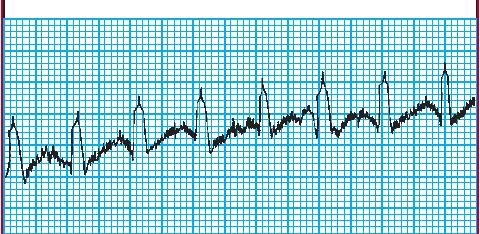
\includegraphics[width=90mm]{figures/ch2/10.png}
	\caption{Electrical interference causes the baseline to be unstable and the signal is corrupted.}
	\label{fig2.10}
\end{figure}

\subsection{Wandering baseline}
A wandering baseline undulates, meaning that all waveforms are present but the baseline is not stationary.  It can be caused by movement if the chest wall during respiration, poor electrode placement, or poor electrode contact.
\begin{figure}[ht!]
	\centering
	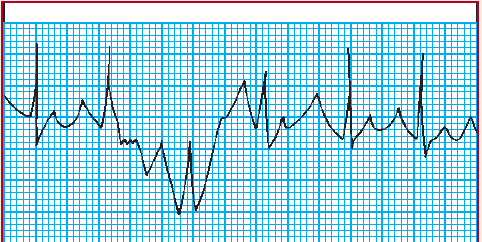
\includegraphics[width=90mm]{figures/ch2/11.png}
	\caption{An example of baseline wandering due to artifacts.}
	\label{fig2.11}
\end{figure}

\subsection{Faulty equipment}
Faulty equipment, such a s broken lead wires and cables, can also cause monitoring problems.
%% Chapter 2

\chapter{State of Art}
\label{Chapter3} 

\section{Device}
The personal health care market has changed a lots and recently new products and devices are showing up on the market. We will describe briefly the most relevant and similar products as mobile ECG acquisition devices.  We evaluate the following solutions:
\begin{itemize}
	\item Mortara ELI 10 Mobile
	\item Philips DigiTrak XT Holter Recorder
	\item M-Trace (PC) Mobile
	\item ECG Expert 
\end{itemize}

\subsection{Mortara ELI 10 Mobile}
This device offers an all in one solution for 12 leads ECG acquisition. It is compact and complete as it provides an alphanumeric keyboard and a screen for real time visualization and the possibility to send the record via GPRS/3G channels. For each devices a SIM card is required . The device can also read and interpret the ECG supporting the doctor. Interesting feature is its great interoperability with the main ECG data management systems.
\begin{figure}[ht!]
	\centering
	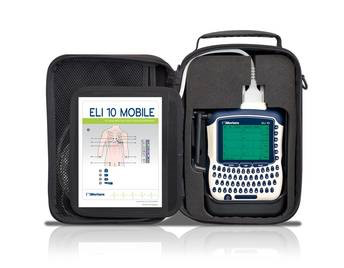
\includegraphics[width=90mm]{figures/ch3/1.png}
	\caption{Mortara ELI 10 Mobile, ECG acquisition device box.}
	\label{fig3.1}
\end{figure}

\subsection{Philips DigiTrak XT Holter Recorder}
This is the smaller acquisition device on the market. Thanks to a proprietary algorithm from Philips it can derive all the 12 ECG leads using only 5 leads. It weighs 62g and the internal battery lasts till 7 days. It also has a small screen showing 1 real time signal at a time.
\begin{figure}[ht!]
	\centering
	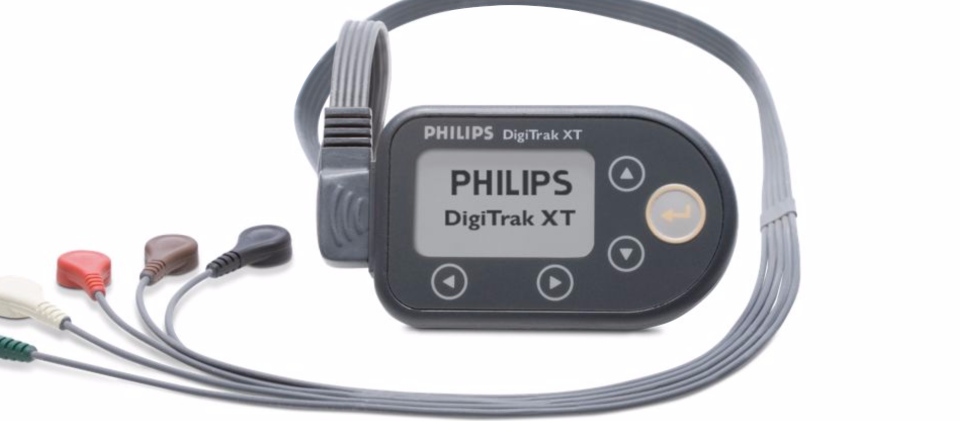
\includegraphics[width=90mm]{figures/ch3/2a.png}
	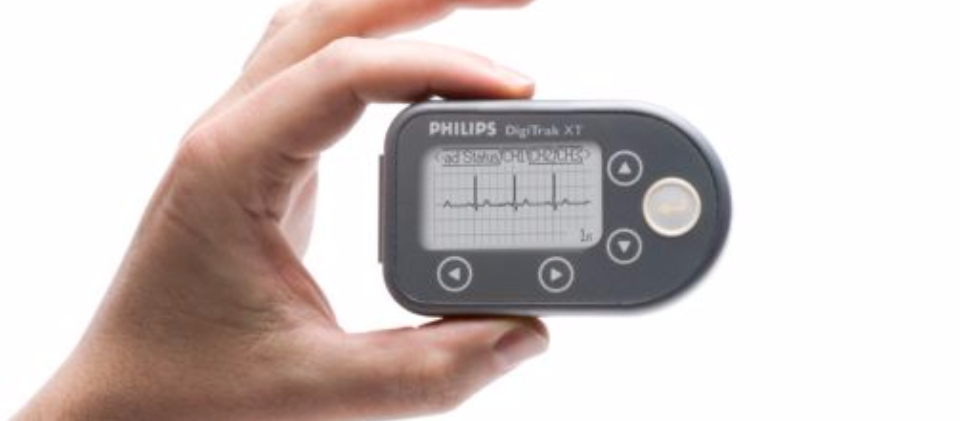
\includegraphics[width=90mm]{figures/ch3/2b.png}
	\caption{DigiTrack, the ECG visualization.}
	\label{fig3.2}
\end{figure}

\subsection{AliveCor ECG}
An innovative solution even though it doesn’t offer a complete solution for ECG acquisition and analysis. This small sensor can be attached on the back of your smartphone making it an ECG acquisition device. It can record only one ECG signal (D1), so also the analysis is limited to a few types of arrhythmias . The record length is also limited to 5 minutes.
\begin{figure}[ht!]
	\centering
	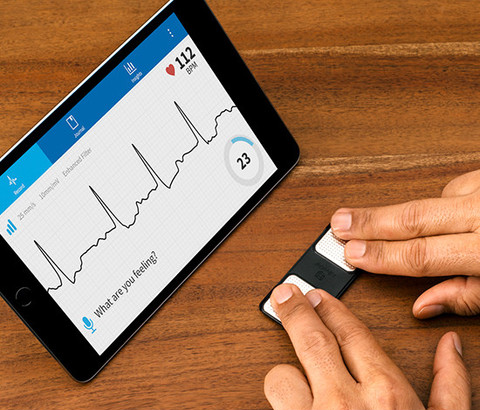
\includegraphics[width=90mm]{figures/ch3/3.png}
	\caption{AliveCor device real time acquisition on a tablet.}
	\label{fig3.3}
\end{figure}

\subsection{M-Trace (PC)Mobile}
M-Trace PC is an completed 12 leads ECG acquisition device. With the device it comes a mobile application and a desktop pc application used to visualize and analyze the ecg signals. The device is really portable with dimensions 95x64x28mm.  The company offers also a more portable device (M-Trace Mobile) to be used by privates at their home. The mobile version cannot acquire a full record but only test records with 6 leads. Its main purpose it to send the test records via GSM/GPRS to the doctor for a faster review.
\begin{figure}[ht!]
	\centering
	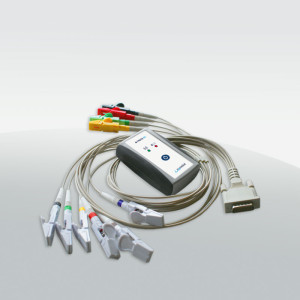
\includegraphics[width=60mm]{figures/ch3/4a.png}
	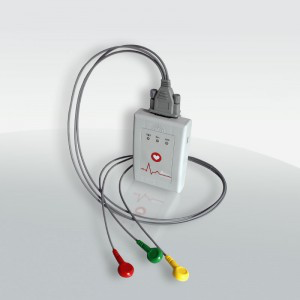
\includegraphics[width=60mm]{figures/ch3/4b.png}
	\caption{M-Trace PC device for ECG acquisition.}
	\label{fig3.4}
\end{figure}

\subsection{ECG Expert}
ECG Expert produced by CSE Medical is a completed solution for ECG acquisition. The device comes with fully supported software for both PC desktop (Windows and Mac) both smartphones  (Android, iOS). The device is rechargeable and makes use of a wireless connection via Bluetooth as exchanges data communication with the handheld smartphone or PC software.
\begin{figure}[ht!]
	\centering
	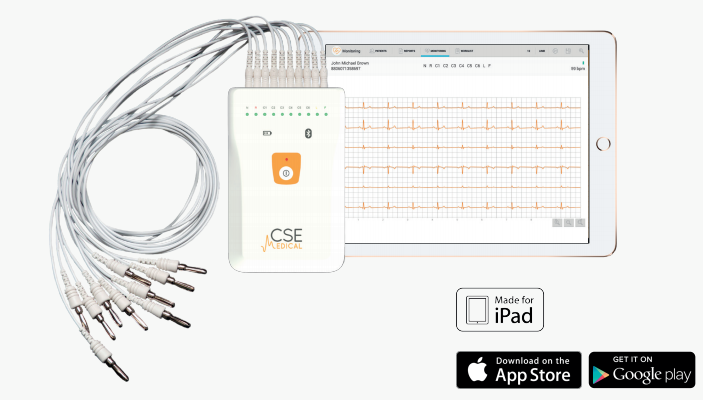
\includegraphics[width=60mm]{figures/ch3/5.png}
	\caption{M-Trace PC device for ECG acquisition.}
	\label{fig3.5}
\end{figure}

\section{Mobile application}
There are already mobile applications on the market store for ECG visualization and analysis supporting different formats. We can distinguish applications that only visualize the signal and the ones that also apply some analysis on the ECG signals. We listed only applications on the Google Play Store, so only Android applications because they are the only comparable with the solution we propose.

\subsection{Visualization only application}
The application on the market able to visualize the ECG signal are:
\begin{itemize}
	\item \textit{StribogECG}: an Android application based on an open source project under GLP v3 licence. It uses Biosig library to read ECG formats such as scp, xml (hl7), ecg and dgf. The software is only provided as it is and it requires to the user to already have the ecg files stored in those supported formats.
	\item \textit{AndroidECG}: application on beta release, it was developed by Paco Gonzàles as thesis project during the Master course in Computer Science at the University of Murcia. The application is able to show ECG signals of the following formats: binary, scp, 212. As additional feature it is a basic analysis over the signal to detect QRS complex, P waves, ST segments and T waves. It is also possible to send the ECG record via email.
\end{itemize}

\subsection{Visualization and Analysis}
The applications on the market that also provide a more detailed analysis over the ECG signal are all bind to a specific proprietary acquisition device. By this way they lack the compatibility and interoperability requirement with other software and ECG formats.
\begin{itemize}
	\item \textit{M-Trace PC}: the application was developed by \textit{M4Medical}, a Poland company providing medical devices for professionals and private customers. The application only works with the company 12-channel ECG M-Trace PC register device. The main features are the real-time monitoring interface, a patients’ database management system and the possibility to share the record.
	\item \textit{ECG Expert}: developed by \textit{CSE Medical} the application works only connected to an ECG-Expert acquisition device. The main features are the real-time view of the acquisition, the analysis of the record providing information about QRS complex and heart rate, the possibility to manage patient information bind to the record and a heartbeat Normal/Abnormal classifier.
\end{itemize}
One last mobile application, which is not strictly related to ECG signal visualization and analysis but it worth to be mentioned, is the \textit{ECG Interpretation}. This application instead provides  enough detailed information about how to read and interpret the ECG signals through 32 small lectures. All the lectures provide a picture and a short description and explanation.
%%Chapter4
\chapter{Objective}
\label{Chapter4} 

\section{Preface}
For a clear understanding of the next chapters we will make use of some terms listed below with the proper meanings:
\begin{enumerate}
	\item Mobile application: it is a software running on smartphones and tablets
	\item Desktop application: it is a software running on desktop pcs or notebooks
	\item Acquisition device: named ZEcg, it is the device (hardware) used to acquire the ECG signal from the electrodes connected to a patient body.
\end{enumerate}

\section{Fully functional medical mobile app as replacement to desktop app}
The main purpose for this thesis is to develop a medical  mobile application as replacement to an original desktop application. The application needs to be standalone and independent from other software, still it can share its content and integrate other software content.\\
As a starting point we planned to reproduce all the desktop features such as the connection between the application and the remote device ZEcg for the ECG signal acquisition. It should also save the ECG records inside the mobile device, plot the signals and run arrhythmia recognition algorithms on them.  We are aware that the user experience is different from a desktop one due to the differences in capabilities and functionalities. Having in mind these differences, we did not try to reproduce the desktop experience. We developed instead the application having a mobile experience at first position, following the standards of mobile application designs and principles. We took advantage of the new and latest technologies mounted on the new smartphones, trying to provide to the end user the best in term of user experience, performance and application design. The main difficulty is probably to redesign and re-imagine the desktop feature from a mobile point of view. For example, if a desktop application usually makes use of keyboard and mouse, inside a modern mobile application there is only the touch input as user interaction. The differences in term of screen size, memory and CPU performance matters and should always be kept in mind during the initial planning phase. We will deal with these and others limitations, trying to achieve the best results and performances. \\
We believe this application can be really a replacement to a desktop application as the technology trend points to future devices with better performances in term of lower power consumption and higher operational capabilities.\cite{ref2}



%%Chapter5
\chapter{Requirement}
\label{Chapter5}
In the project there was the need for a deep analysis of all the tied requirements. The result of this analysis was essential to identify the subsequent problems.\\
We will describe all of them, distinguishing between functional and nonfunctional requirements.
\section{Functional}
\subsection{Connection management with the acquisition device}
Fundamental feature to be included inside the mobile application is the capability to directly connect the smartphone device to the acquisition device ZEcg. Since this last one was designed to transmit the signals through a bluetooth channel, we have to implement and manage a bluetooth socket connection inside the application in order to receive the data.
\subsection{Acquisition, storing and management of ECG records}
For a matter of medical feature as it is a fact that there are many “standards” on saving an ECG signal, the application has to be able to manage different formats. Even though this application is designed to be used mostly for acquisition from the ZEcg device, it is also able to open and read other standard format such as the MIT-BIH, one of the most common standard in the literature of ECG. The code software behind is designed in a such  way that the integration of other format is made extremely easy to add just by implementing few interfaces and classes.

\subsection{Different ECG formats support}
For a matter of medical feature as it is a fact that there are many “standards” on saving an ECG signal, the application has to be able to manage different formats. Even though this application is designed to be used mostly for acquisition from the ZEcg device, it is also able to open and read other standard format such as the MIT-BIH, one of the most common standard in the literature of ECG. The code software behind is designed in a such  way that the integration of other format is made extremely easy to add just by implementing few interfaces and classes.

\subsection{Dynamic display scaling}
The mobile device market is huge and there are a very large number of devices with completely different hardware and screens. As first classification we can distinguish mobile devices into smartphones and tablets. The most obvious difference is based on the screen size and the pixel density. Building a mobile application means also to deal with these number of different devices. To achieve the same experience and look and feel the application should be able to scale its view according to the device screen and the pixel density. A typical ECG signal is plot on a paper with squares of well defined size in millimeters. The mobile application has to respect such a standard independently on the screens capabilities and pixel density, so it should be able to properly scale the view and the plotting based on the hardware provided by the device.
\subsection{ECG record analysis integration on mobile platform}
To complete the set of features for the application we plan to integrate the algorithms of ECG signal processing. To have a mobile device able not only to acquire and visualize in real time the ECG but also to analyze it at runtime, can be of vital importance, especially if the user has little knowledge about reading and interpreting an ECG graph. The integrated algorithms for arrhythmia analysis are based on a Neural Network trained to recognized the nature of the signals for the given record with high accuracy. The algorithms come from a previous thesis work\cite{ref3} which belongs to Ulisse Pizzagalli, student at Politecnico of Milan.
\subsection{Analysis results displaying}
After analysis there are results that need to be shown to the user in the most friendly and understandable way. The most important results from an ECG analysis are called Istogram, Tacogram and the ST+/ST- . They are respectively graphs showing the number of heart rates of a certain value, the average heart rate at each heart beat and the difference between the area ST+ and ST-, the area above the segment ST and the one below. This last graph is useful for ischemia detection.\cite{ref4}
\begin{figure}[ht!]
	\centering
	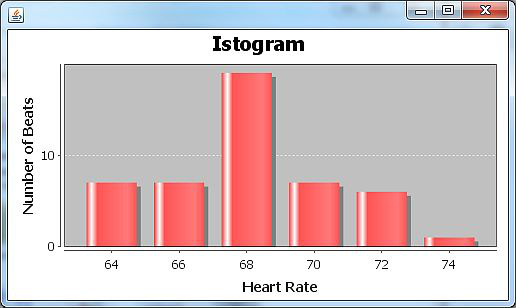
\includegraphics[width=90mm]{figures/ch5/1.png}
	\caption{Istogram from the desktop application resulted from an analysis on a MIT/BIH record.}
	\label{fig5.1}
\end{figure}
\begin{figure}[ht!]
	\centering
	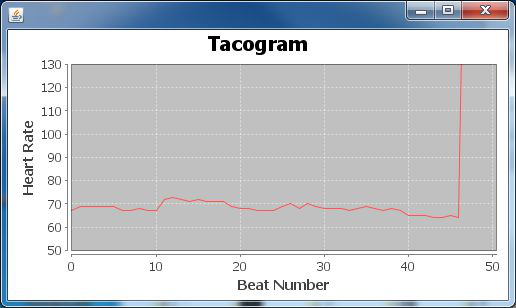
\includegraphics[width=90mm]{figures/ch5/2.png}
	\caption{Tacogram from the desktop application resulted from an analysis on a MIT/BIH record.}
	\label{fig5.2}
\end{figure}
\begin{figure}[ht!]
	\centering
	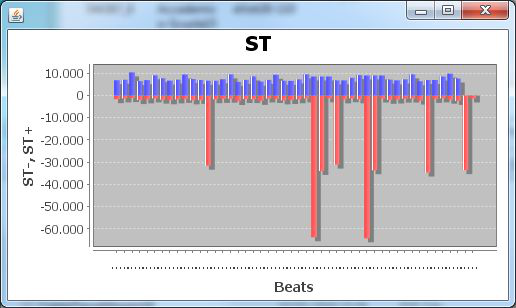
\includegraphics[width=90mm]{figures/ch5/3.png}
	\caption{ST+/ST- graph from the desktop application resulted from an analysis on a MIT/BIH record.}
	\label{fig5.3}
\end{figure}
\subsection{Highly parameterizable}
We believe in dynamic software, that is why we planned from the beginning on making this application dynamic. Even if the application is  build on top of the ZEcg standard, we plan to make the software responsive also to other standards. To achieve this, we planned to abstract all the acquisition device independent features and functionalities. In order to support as much as possible any variants of the original acquisition device, we plan to setup customizable parameters, the only related to the hardware implementation. With a little of changes the application will be able to interface with other devices as well for acquisition.
\section{Nonfunctional}
\subsection{Reduced memory usage}
This requirement is fundamental for any project related to mobile application development. In fact, if a desktop pc in general doesn’t have any problem related to memory usage (even if it is a good practice not to waste memory), on mobile devices this over-usage can bring the application to crash and get killed by the OS. The memory available is higher on new devices with respect to older ones,  but it is still small so it is always a good practice to use it carefully.
\subsection{Minimum performance rate and scalability on performance}
Nowadays the new high level mobile devices has quad-core or even octa-core cpu processors. Any application should take advantage of a such configuration, but on the other hand mobile application developers should always consider the fact that the market is still full of older and low-end devices. In order to cover at least most of the market devices their application have to run fine (with a minimum acceptable performance rate) starting from the low-end devices and, at the same time, taking advantage of last devices capabilities. \\
We believe modern applications should seriously take this aspect in consideration, because it will make their application scalable also from a performance point of view.
\subsection{ Wide platform compatibility and accessibility}
Developing a mobile application implies building a software that has to be executed on many different platforms. The smartphone and tablet market is huge with many different devices mounting different hardwares and running of the three major mobile OS (iOS, Android and Windows Phone). In the next chapters we will deal with this issue.   
\subsection{Documentation}
This thesis includes also a more technical documentation about the development phase and the choices we starting from the planning phase to the development phase. The software is fully documented and with annotations and comments to increase code readability and future development on top of it. The technical documentation is included in the next chapters where we are going to discuss and motivate the implementation and the results.

\backmatter
\newpage \thispagestyle{empty} \newpage 

%------------------------------------------------ Acknowledgements

% Page without header
\newpage \thispagestyle{empty} \newpage 
\chapter{Acknowledgement}
\setlength{\parskip}{0.8em}
\begin{flushright}
\textit{
	To my parents, mother Stella and father Gregorio who are always the fixed stars in my sky.\\
	To my brother Dung who is in my blood.\\
	To Dora who is in my deeper heart.\\
	To all my best friends who may be physically far away but I know they will answer to any my calls.
	To all the ones who never believed on me.\\
	Thanks to all of them I am the man I wished to be.\\
	The future is a step ahead and thank to my beloved supporters I am not scared to go further\dots
}\\
\textbf{Chai}
\end{flushright}

\textit{
	To my family and all my friends.\\
	To the destiny.	To God\dots
}\\
\textbf{Antonello}

\setlength{\parskip}{0em}

\bibliography{Include/Bibliography}

%\include{Appendix}

\end{document}
